%%%%%%%%%%%%%%%%%%%%%%%%%%%%%%%%%%%%%%%%%%%%%%%%%%%%%%%%%%%%%%%%%%%%%%%%%%%%%%%%
%
% FILE: font_free_ocr.tex
%
% DESCRIPTION: LaTeX source file of ICDAR 2007 paper submission
%
% CVS:
% $Id: font_free_ocr.tex,v 1.16 2007-02-04 01:20:43 scottl Exp $
%
%%%%%%%%%%%%%%%%%%%%%%%%%%%%%%%%%%%%%%%%%%%%%%%%%%%%%%%%%%%%%%%%%%%%%%%%%%%%%%%%

% INITIALIZATION %
%%%%%%%%%%%%%%%%%%
\documentclass[times, 10pt,twocolumn]{article} 
\usepackage{latex8}
\usepackage{times}
\usepackage{graphicx}
\pagestyle{empty} %remove page numbers

% DOCUMENT START %
%%%%%%%%%%%%%%%%%%
\begin{document}

% TITLE %
%%%%%%%%%
\title{Shape-Free Statistical Information in Optical Character Recognition}

% AUTHOUR INFO %
%%%%%%%%%%%%%%%%
\author{First Author\\
Addr 1\\
Addr 2\\
Addr 3\\
\and
Second Author\\
}

%@@the following is not to be included during the review process
%\author{Scott Leishman\\
%Department of Computer Science\\
%University of Toronto\\ 
%scottl@cs.toronto.edu\\
%\and
%Sam Roweis\\
%Department of Computer Science\\
%University of Toronto\\
%roweis@cs.toronto.edu\\
%}

\maketitle
\thispagestyle{empty}


% ABSTRACT %
%%%%%%%%%%%%
\begin{abstract}
We introduce an approach to character recognition that does not rely on shape 
or font information, instead decoding the sequence of clustered ink blobs by
exploiting word positional statistics, and dictionary lookup information.
Applying this procedure to a test set of 10 long documents yields an average
character recognition accuracy performance above 90\%, and above 88\% on a set 
of 159 perfectly clustered short documents.
\end{abstract}


% INTRODUCTION %
%%%%%%%%%%%%%%%%
\Section{Introduction}

Traditional approaches to optical character recognition have typically
relied on font-specific shape information to convert bitmap
images of glyphs into corresponding sequences of (ASCII or Unicode encoded)
characters.  Some of the earliest systems were heavily restricted, only
able to recognize images that happened to closely match a template culled from
a database containing a handful of common typefaces in typical point
sizes.  Modern systems have improved, and are now able to recognize
symbols from a much larger collection of varying fonts and character shapes.  
This has often been accomplished by using images or features of images from a 
wide array of font faces, styles, and sizes as labelled training data for 
training character classifiers.  Nonetheless, performance still degrades
in documents containing unusual typefaces or fonts sizes.  
As electronic publishing becomes increasingly common (including the
ability for ordinary users to create their own custom fonts), the enormous
variety of fonts seen in printed and online documents continues to grow rapidly.
This creates an ongoing motivation to pursue sources of {\em font and shape
independent} information useful for optical character recognition.

Many previous attempts at ``font free'' character recognition share
the same general structure.  Each page of ink is segmented into components
roughly corresponding to individual graphemes of the 
underlying document language. These components are clustered together in an 
unsupervised fashion based only on visual similarity.  (For a language like 
English, the ideal result of this step would be a set of clusters such that
each one contains only occurrences of a particular 
character, digit, or punctuation symbol found in the document.
Of course, such exact clusterings are rarely achievable in practice, and 
trade-offs must be made between the final number of clusters and the 
consistency of the component members within a cluster.)
In one of the earliest shape-free recognition approaches, Nagy et al. treated
the clustered sequence of components as the input cipher-text of a 
cryptogram\cite{nagy1987}.  Clusters were then assigned plain-text labels, 
with the assignment guided by the frequency of matches to words looked up in a 
small dictionary.

Building on this, Ho and Nagy attempted to infer cluster labels using a series 
of simple statistical modules\cite{ho2000}.  Each module scores potential 
assignments using what they call a ``v/p ratio'', which counts the number of 
valid dictionary words that match the partially assigned word patterns that 
contain the cluster to be mapped.  In subsequent work, they used 
several n-gram, frequency, and word-positional features to construct a 
classifier able to reliably determine whether an appropriately segmented 
cluster was an upper or lower case character, a digit, or a 
punctuation symbol\cite{ho2001}.

Recently, Huang et al. have used an entropy based approach to decode the
sequence of cluster identifiers representing individual words\cite{huang2006}.  
Confident mappings (those for which the distribution over character labels is 
sharply peaked at just a single label, given a dictionary of lookup words the 
same length as those that the cluster to be mapped appear in) are assigned 
first and used to narrow down the mappings for subsequent clusters.

In this paper we explore the extent to which contextual and statistical sequence
information can be exploited in character recognition without making any
a priori use of character shape or font knowledge. We extend earlier
investigations by reporting results on all character types, not just
lowercase alphabetic characters. As well, we provide an analysis of
cases in which purely contextual information is not sufficient to
establish character identity.


%unfortunately this figure has to be moved to get it to appear on the same page
%as its description.
\begin{figure*}[ht]
  \centering
  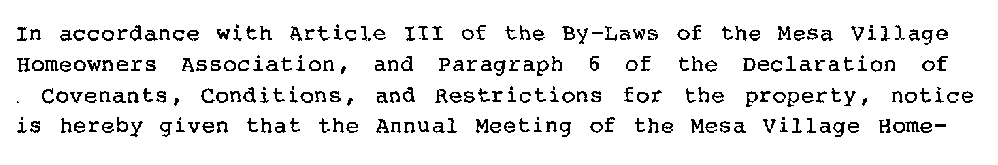
\includegraphics[scale=.7]{figures/input_lines}
  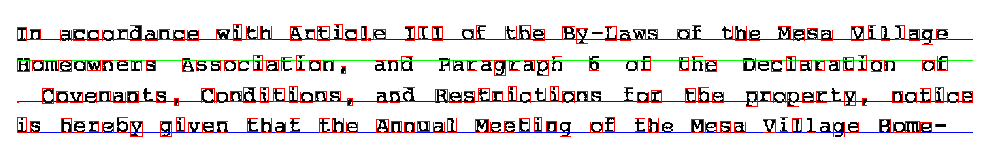
\includegraphics[scale=.7]{figures/line_comps}
  \caption{Sample input image region and corresponding components, baselines,
           and x-heights found}
  \label{inimg_fig}
\end{figure*}

% CLUSTERING APPROACH %
%%%%%%%%%%%%%%%%%%%%%%%
\Section{Clustering Procedure}
\label{clustering_sec}

Before attempts can be made to recognize the sequence of glyphs that 
constitute input document images, the appropriate elementary symbol regions 
must first be located, isolated, and clustered together.\footnote{The
discussion that follows assumes the document images given are not
already ``symbolically compressed''. Such a compression scheme will
store a single template image and the offset locations of each
appearance of that particular shape, even grouping together
those shapes that are slightly varied.  For input document images that
have been compressed in this way (via a JBIG2 compliant encoder 
or parsing a PDF file for instance), a clustering procedure is often not necessary.}
After typical page image preprocessing steps like layout analysis, textual
region identification, and deskewing, are performed, the
connected components of ink are identified and their bounding box
positions on the page are stored.  For each component, the nearest neighbouring
component in each of the four principal directions (top, bottom, left, and
right), as well as pixel offset distance are also stored.  Individual lines
of text are then identified by following the chain of neighbouring components in
reading order.  The bounding box for a line is expanded as neighbour
component positions are read, and checks are made of neighbours in non-reading
order directions to determine if a line should be extended perpendicularly.
%
Since some symbols like {\tt i, \'{e}, :, ?} are made up of more than one
connected component, attempts are made to merge their constituent parts.  This
is accomplished by looking for separate components that belong to the same
line, are separated by a relatively small vertical distance (set manually), and
have one of the components completely overlapping the other horizontally.

Figure \ref{inimg_fig} illustrates this line and component finding process on a
small region of input text (top).  The bottom half of the figure shows that on
this particular region, almost every connected component corresponds to a
single character glyph.  The baseline and x-height of each line found is also
shown.

Each connected component image is initially assigned to its own cluster, then
clusters are merged in an agglomerative fashion.  First a simple Euclidean
distance measurement is taken between cluster centroid images, and those whose
value falls below a conservatively set threshold are merged together.  For near
noiseless documents with consistent symbol shapes, this has the effect of 
greatly reducing the number of clusters in a fairly efficient manner.
The clusters are subsequently refined using the
Hausdorff distance\cite{rucklidge1996}.  Because the cluster average images 
may not be binary, they are first thresholded so that they can be compared using
this metric.  Those that fall within a particular threshold ($\sqrt 2$ in our
experiments) are then clustered together.  Figure \ref{hausdist_fig}
shows this calculation between a lower case {\tt e} and a lower case {\tt o}, 
and between the {\tt e} and an italicized version of the same character.  The 
Euclidean distance transform is calculated with the resultant values listed for 
each pixel, and an image of the character to be compared is laid overtop.  The 
on pixel of the comparison character which lies farthest from any on pixel in 
the original character is highlighted. 

\begin{figure}[ht]
  \centering
  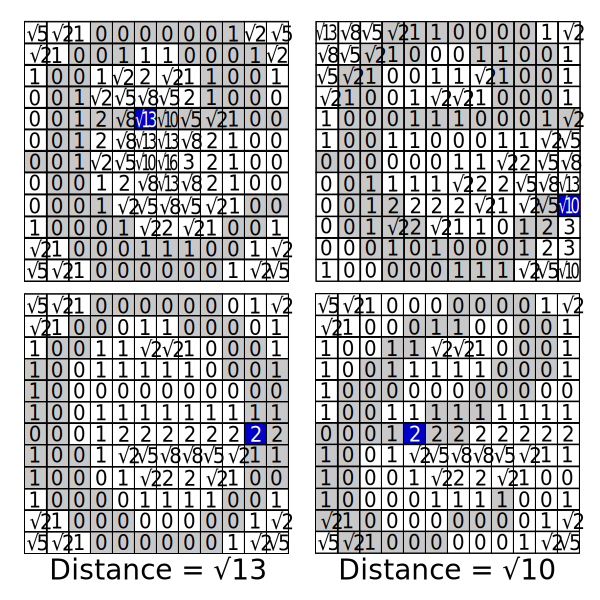
\includegraphics[scale=.4]{figures/haus_dist_comparisons}
  \caption{Hausdorff distance as calculated between a regular and italicized
  {\tt e} versus a regular {\tt e} and an {\tt o} in the same font}
  \label{hausdist_fig}
\end{figure}

It should be noted that no attempts are made to normalize characters since the
Hausdorff distance combined with the averaging that takes place as components
are added to the clusters, can typically handle small deviations in font size.
While this may result in multiple clusters for the same symbol if font sizes
differ drastically, contextual procedures outlined in the following section
should still result in correct symbol recognition for all such clusters.

Depending on the font face, amount of kerning employed, and the quality of the
input document image, some glyphs may be broken into two or more pieces, or
they may end up touching one another resulting in a single component containing
multiple symbols.
To handle glyphs that have been broken apart, we attempt to recombine them by
examining the clusters that they belong to.  If components belonging to a
particular cluster tend to always lie adjacent to components in a second
cluster (and vice versa), and if the typical distance between these components
is relatively small, then they are merged.  In our experiments, those clusters
for which at least 85\% of the components share a neighbouring component in the
same second cluster, and are no farther than 3 pixels apart are merged.

Attempts are made to separate glyphs that have been smeared or so tightly
kerned that they are touching, by iteratively splitting the glyph near a
suspected boundary and trying to match each half with other cluster averages.
Provided both halves lie within a small Euclidean distance of their matching
clusters, the components of the original cluster are split at the appropriate
position, and added to their respective matching clusters.

This Hausdorff matching, cluster merging and splitting procedure is repeated
over those clusters that have had at least one change to their number of 
components at the previous iteration, until no further changes are seen.

With symbol clustering complete, a cluster is created to represent the blank
space between each word of documents written in alphabetic languages.
Inter-word space width is estimated in a simple fashion by counting the
frequency of component neighbour distances.  This distribution is typically
bi-modal with the first mode representing inter-character spacing, and a second
(often smaller) mode representing inter-word spacing.  The width assigned
is based on this second modal point, but is underestimated slightly to ensure no
actual inter-word spaces are missed.  New components are created representing
each of these spaces, and neighbours are updated appropriately.

Figure \ref{clavg_fig} shows the resulting cluster averages after this
procedure has been run on a single document taken from the DOE 3 OCR dataset 
created by ISRI\cite{nartker2005}.

\begin{figure}[ht]
  \centering
  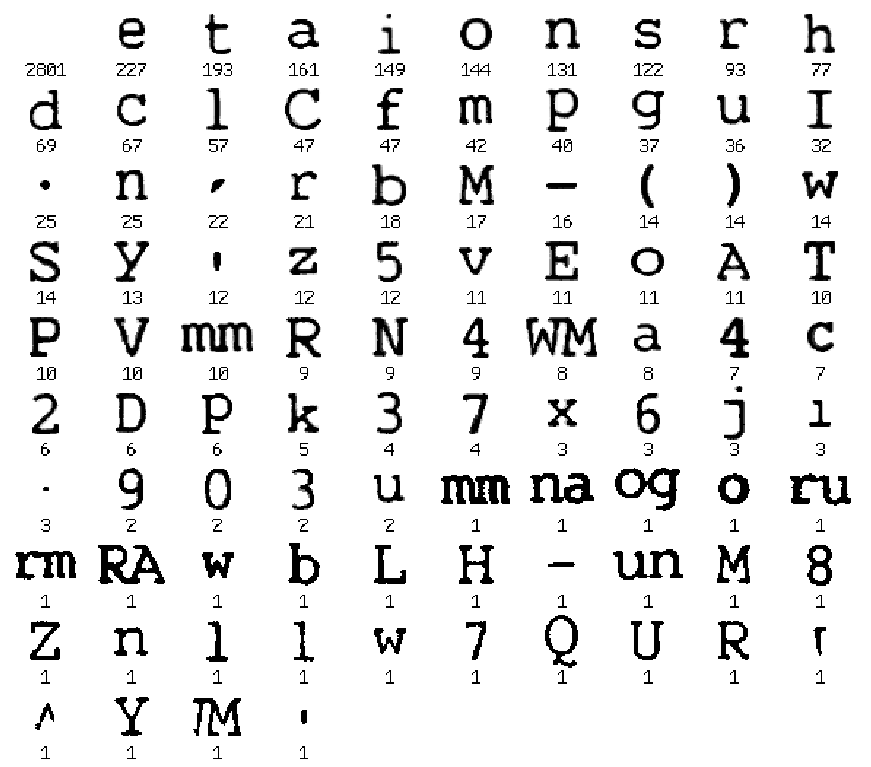
\includegraphics[scale=.4]{figures/cluster_averages}
  \caption{Typical document cluster averages}
  \label{clavg_fig}
\end{figure}


% CONTEXTUAL RECOGNITION APPROACH %
%%%%%%%%%%%%%%%%%%%%%%%%%%%%%%%%%%%
\Section{Contextual Recognition Based on Position}

With a reasonable clustering complete, the labels belonging to each cluster are
ready to be recognized.  Our contextual recognition approach has only been
tested on documents written in English, but should also be amenable to other
writing systems whose atomic symbols are roughly phonetic.  In our experiments
we have also assumed that we know in advance the language of the
input document, however previous research has shown it possible to infer this
automatically with relatively good accuracy\cite{sibun1994}.

First a large text corpus is used to estimate overall word and symbol frequency,
as well as symbol positional frequency.  We take counts of the number of times
each symbol appears in each position of words up to a particular length.  As
a result of this, each symbol will then define a point in an $\frac{x
(x+1)}{2}$ dimensional ``positional'' feature space, where $x$ defines the
maximum word length to include (15 in our experiments).  We normalize the
positional counts for each symbol so that within each word length, we end up
with a distribution over positional frequency.  Figure \ref{e_pos_fig} shows
this resultant feature vector for the symbol {\tt e} when estimated over part of
the Reuters-21578 news corpus\cite{lewis2004}.

We repeat this process on the sequence of clustered components by
gathering positional cluster frequency stats using the estimated
components of the space symbol cluster to demarcate word boundaries.
By taking these counts over words of length $x$ or less, we have that
each cluster can be described as a point in this ``positional''
feature space.

Before comparing cluster feature vectors with those in our symbol
corpus, we first re-weight the symbol feature vectors based on
word-length.  Since most words in the English language are relatively
short, this will help minimize the effect of wild positional
differences in longer words (since there will typically be few long
cluster sequences in short documents).

Determining which symbol each cluster belongs to involves ordering the
observed frequency vector of each cluster in the ``positional''
feature space with the feature vectors for the known characters, as
estimated on a large reference corpus. When the match is almost exact
(in our experiments we use Euclidean distance, but a weighted
cross-entropy could also be applied), we can make an assignment
directly.  For frequently occurring symbols like lowercase vowels or
common consonants, there are often enough counts that the cluster
positional feature vectors closely match the corresponding reference
vector, and so such a match is reliable.  However for
infrequently occurring symbols, feature vectors exhibit high variance
(due to the subject of the document for instance), thus additional steps must 
be taken.

\begin{figure}[ht]
  \centering
  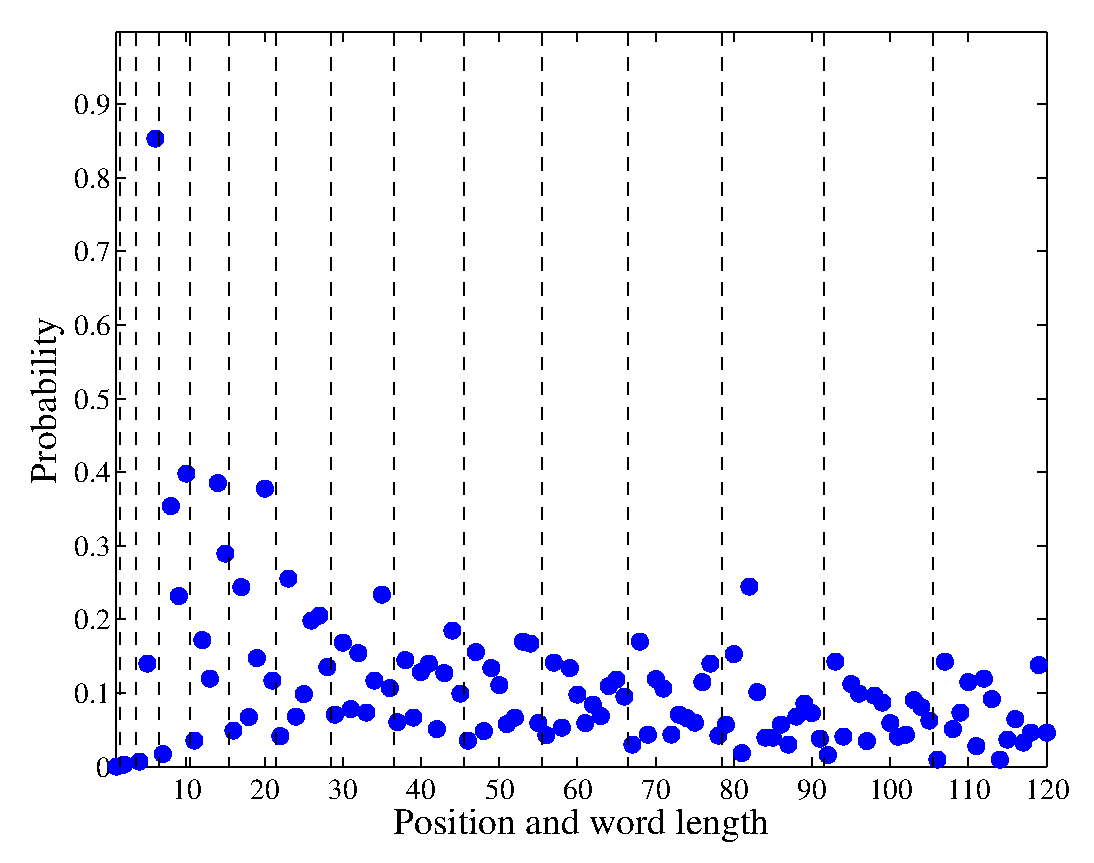
\includegraphics[scale=.5]{figures/e_pos_feature}
  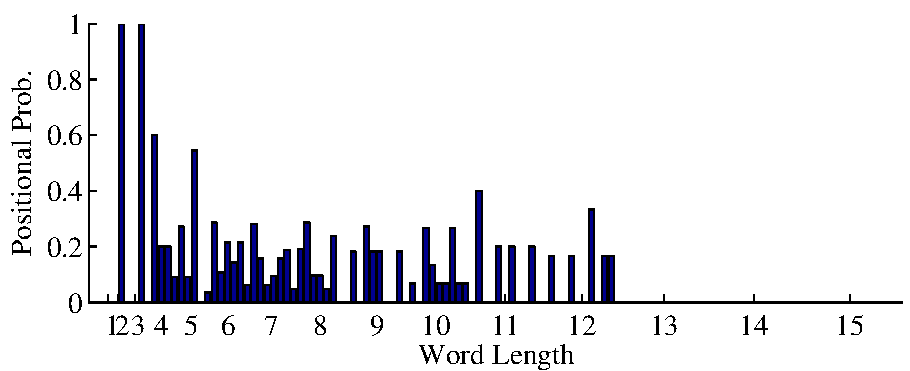
\includegraphics[scale=.5]{figures/e_pos_feature_clust}
  \caption{Reference feature vector for the character {\tt e} (top),
           and its corresponding cluster vector when taken from a short
           document. }
  \label{e_pos_fig}
\end{figure}

We take a greedy approach in which we assign clusters to characters
one at a time, starting with the clusters appearing most frequently in
the document.  For each cluster, we consider the top matching
characters candidates according to the positional feature vector.  For
each candidate, we use the partially assigned mapping so far to match
words containing the current cluster symbol against a large word
corpus from a dictionary. The fraction of total words in the input
document containing the cluster which are matched is calculated and
provided that it exceeds a particular threshold (75\% in our
experiments), then the character candidate under consdieration is
permanently assigned to the cluster, and we move on to determine the
mapping for the next cluster.  Initially, when few symbols have been 
matched, many dictionary words are potential matches for the next cluster. 
As more clusters are assigned symbols, it eventually becomes impossible for
a particular cluster to find a character mapping that achieves a
matching word ratio exceeding the desired threshold.  In such a case,
the symbol that achieves the largest such ratio is taken to be the
correct mapping.  If multiple symbols generate the same dictionary
lookup ratio, then ties are broken by first using line offset information 
to reduce the number of symbols.  Each symbol and cluster is classified as
one of 4 types based on its ascender and descender offsets.  If multiple
symbols from the same class match, then the symbol with a closer positional
feature distance is chosen.  This process is repeated until each cluster has 
been assigned a symbol.


% EXPERIMENTS %
%%%%%%%%%%%%%%%
\Section{Experiments}

To examine the information present in positional statistics, we have completed
experiments using the fine-mode fax quality images from the business letter, 
and legal document ISRI OCR datasets\cite{nartker2005}.  All 159 documents from
the business letter set, and the 10 longest documents (labelled 9460-9469) were
taken and deskewed using the library included with the Leptonica image
processing suite\cite{bloomberg2006}.

Dictionary word lookup, and output symbol positional statistics were estimated
from the first piece of the Reuters-21578 news corpus 
(reut2-000.sgm)\cite{lewis2004}.  Each article's body text was extracted and the
trailing ``Reuter'' byline was removed, leaving a total of 744,522 symbols, and
17,601 unique words (including many proper nouns, digit strings, and words with
punctuation symbols).  Our output alphabet consisted of 92 different symbols
including upper and lowercase letters, the digits 0-9, punctuation, brackets, 
and several simple arithmetic operators.

To test overall performance on short, low quality documents, the images from
the business letter dataset were used.  These documents were typically only 1
page in length, and contained 2010 characters on average.  84.2\% of all
characters were lower case letters, 8.52\% were upper case letters, 3.29\% were
digits, and the remaining 3.99\% were punctuation or other symbols.

After grouping the pages belonging to each document together and clustering 
the images using the procedure described in Section \ref{clustering_sec}, 
positional features were then calculated for each cluster.  These feature 
vectors were compared with the feature vectors found for the output 
symbols, which were weighted based on how frequently words of that length 
appeared in the corpus.  The resultant distances were used to define an 
ordering of output symbols for each cluster.

To determine the final mapping for each cluster, vp-ratio scores were
calculated for the first symbol in the order given the partially assigned
mappings up to that point.  If it was found that this score exceeded a 
threshold of 75\%, the mapping was deemed correct, otherwise vp-ratio scores
were calculated for all symbols in order, and that which acheived the maximum
was taken.  Ties amongst vp-ratio scores were broken by taking the output
symbol with a closer positional feature distance.  This final mapping was then
combined with the cluster sequences found to generate output text, which was
compared against the corresponding ground truth to determine accuracy.

Accuracy was established for symbols on a per-class basis (lower case letters, 
upper case letters, digits, and punctuation and other symbols).  Word accuracy
counts were also taken.  Table \ref{acc_tbl}, column 'B' shows the 
resultant performance when accuracies are averaged across all 159 documents.

To examine the effect clustering performance had on the achieved accuracy,
tests on the business letter dataset were re-run using the ASCII codes of the
ground truth text.  Symbols were grouped together provided they had the same
code, allowing us to assess performance on a perfectly segmented and clustered 
set of data.  As in the previous test, positional feature statistics were
computed, and compared against those from the same corpus, and vp-scores were
used to determine final mappings.  Table \ref{acc_tbl}, column 'B (ASCII)'
shows the resultant improvement in accuracy.

To determine the impact that document length has on performance we also tested 
our approach on the longest documents in the legal document dataset.  Each of 
these documents was 15 pages in length, and averaged 22,959 characters.
90.74\% of all characters were lower case letters, 4.55\% were upper case 
letters, 1.68\% were digits, and the remaining 3.03\% were punctuation or 
other symbols.  Results are reported when clustering the input images, and 
when using the ASCII codes, and are reported in the 'L', and 'L (ASCII)' 
columns of Table \ref{acc_tbl} respectively.

\begin{table}[ht]
  \begin{tabular}{|c|c|c|c|c|}
    \hline
    & B & B (ASCII) & L & L (ASCII)\\
    \hline
    \hline
    overall & 67.84 & 88.24 & 90.72 & 96.07\\
    \hline
    low letters & 73.17 & 95.71 & 97.79 & 100\\
    \hline
    upper letters & 9.21 & 50.65 & 4.02 & 65.66\\
    \hline
    digits & 6.84 & 20.52 & 7.51 & 23.64\\
    \hline
    other sym. & 24.55 & 52.36 & 31.44 & 61.72\\
    \hline
    word & 50.50 & 79.91 & 92.49 & 95.30\\
    \hline
  \end{tabular}
  \caption{Recognition Accuracy based on symbol type for image and ASCII code
           clustered data}
  \label{acc_tbl}
\end{table}

To further illustrate performance versus document length, the per class
accuracies of each document in the business letter dataset was plotted.  The
results are shown in Figure \ref{acc_v_doclen_fig}.

\begin{figure}[ht]
  \centering
  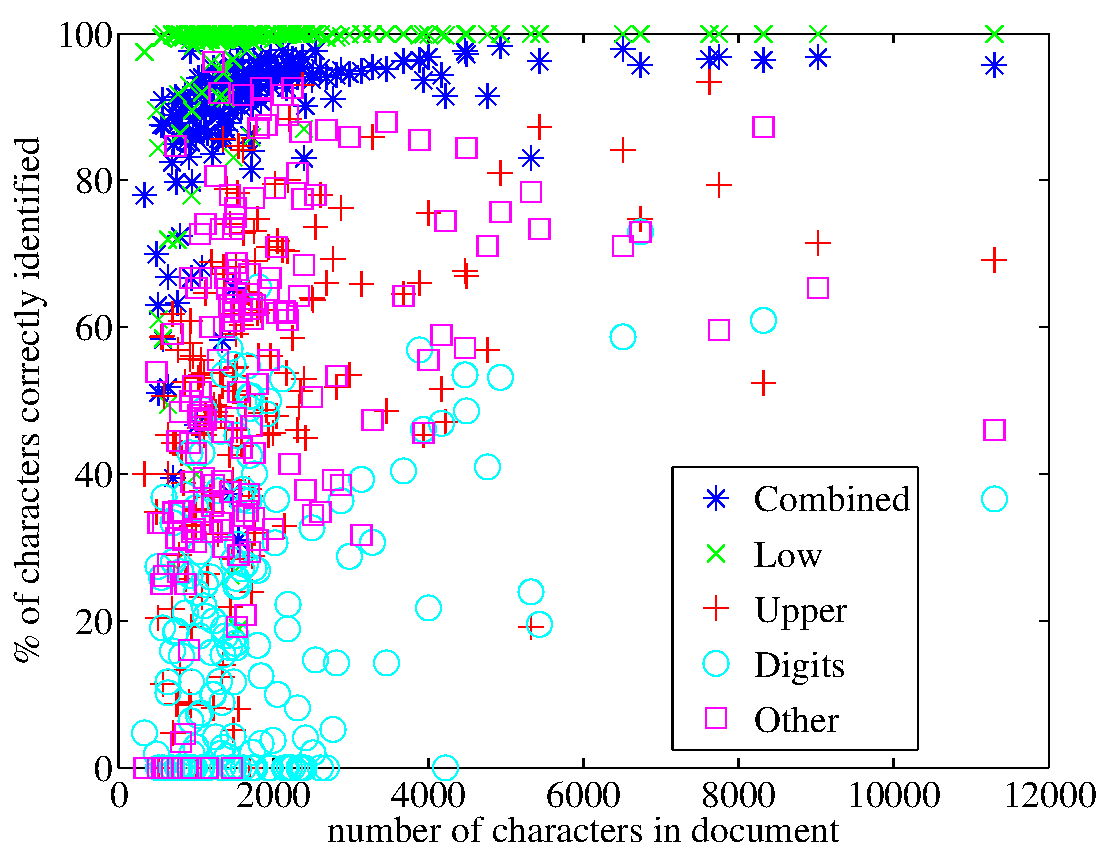
\includegraphics[scale=.4]{figures/acc_v_doclen}
  \caption{Percentage of ASCII codes correctly recognized versus document
  length from the business letter dataset}
  \label{acc_v_doclen_fig}
\end{figure}

% CONCLUSIONS %
%%%%%%%%%%%%%%%
\Section{Conclusions}

We have found that given an ideal segmentation and clustering of the input
data, contextual information alone can lead to fairly strong results for lower
case letters, even on short documents.  For the remaining symbol classes, they
suffer from not belonging to words in the lookup lexicon, as well as
having skewed positional features owing to their relative infrequency in shorter
documents.  While a large lookup dictionary may help with the former, another
source of information will most likely be required to help with the latter.

Our results also highlight the importance of an accurate segmentation and
clustering procedure.  Significant information was lost when multiple symbols
were merged or broken apart, and inaccurate estimation of intra-word space
length was shown to yield particularly poor performance as broken words would
significantly alter word lookup scores and mapping choices.


% REFERENCES %
%%%%%%%%%%%%%%
\bibliographystyle{latex8}
\bibliography{font_free_ocr}

\end{document}
